\subsection{Menu principal}
Cuando inicias \emph{Granny's Bloodbath} comienzas en el menú principal. Con las teclas de dirección puedes moverte por las distintas opciones:

\begin{center}
	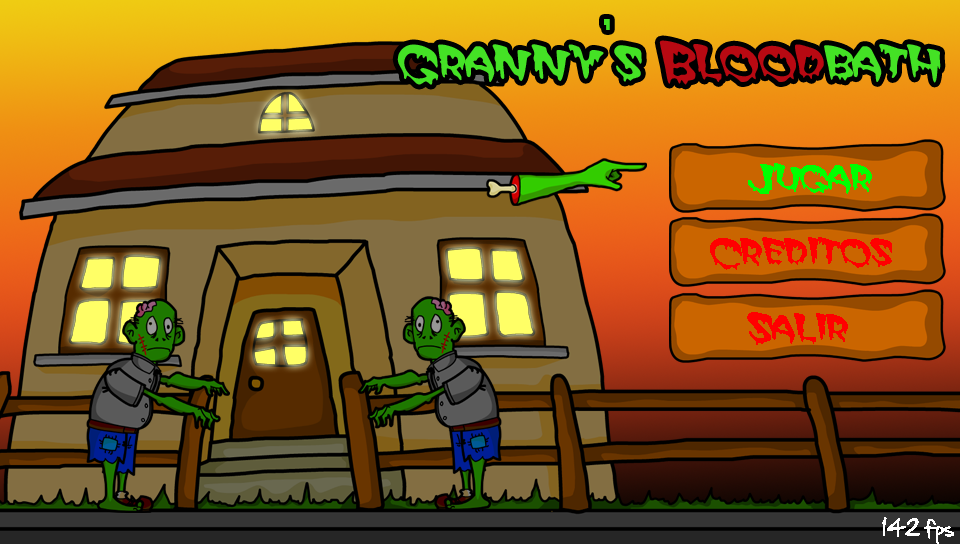
\includegraphics[scale=0.35]{screen-menu.png}
\end{center}

\begin{itemize}
	\item \emph{Jugar:} comienzas una nueva partida o continuas la que habías dejado a medias
	\item \emph{Créditos:} puedes ver las grandes personas que han desarrollado o contribuido a desarrollar \emph{Granny's Bloodbath}
	\item \emph{Salir:} cierras el juego pero no quieres eso, ¿verdad?
\end{itemize}

Para seleccionar una pulsa la barra espaciadora.

\subsection{¡Quiero jugar!}
Bien, has elegido comenzar la aventura. En \emph{Granny's Bloodbath} existen dos tipos de escenas: las de historia y las de juego. 

\begin{itemize}
	\item \emph{Escenas de historia: } se nos cuenta algún fragmento de la aventura de nuestra abuelita. Podemos escuchar al narrador o pulsar \emph{ESCAPE} para avanzar.
	\item \emph{Escenas de juego: } la acción, la sangre y toda la diversión se encuentran concentradas en los niveles del juego. A continuación explicamos el significado de los indicadores que aparecen en pantalla así como los controles para manejar a la abuelita. Si lo que quieres es crear tus propios escenarios debes avanzar un poco más.
\end{itemize}

Cuando comiences a jugar verás una pantalla semejante a esta:

\begin{center}
	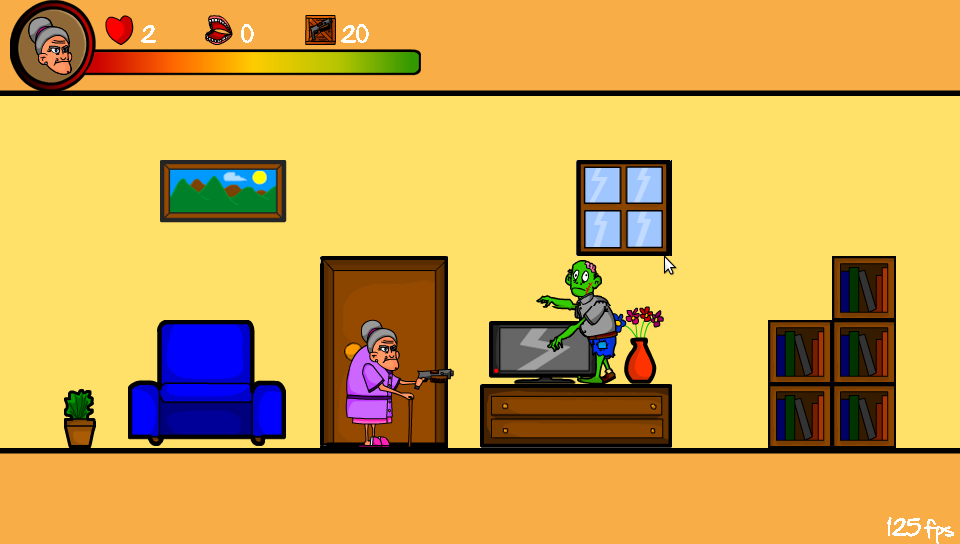
\includegraphics[scale=0.35]{screen-juego.png}
\end{center}

\subsubsection{HUD}
El HUD es la zona donde se encuentran los indicadores que nos informan sobre el estado de la abuelita. Tiene los siguientes componentes:

\begin{center}
	
\includegraphics[scale=0.35]{hud.png}
\end{center}

\begin{itemize}
	\item \emph{Barra de vida}: Disminuye con los ataques zombie, ¡ten cuidado, si llega a 0 perderás una vida!
	\item \emph{Corazones}: Número de vidas disponibles. Si te eliminan y te quedan vidas volverás a empezar el nivel pero si no te quedan tendrás que empezar la aventura desde el principio.
	\item \emph{Dentaduras}: Puntos, si consigues un número determinado se te obsequiará con una vida adicional
	\item \emph{Munición}: La munición de la escopeta es limitada, ten cuidado, no la malgastes y consigue todas las cajas de munición. Disparar a distancia es una gran ventaja.
\end{itemize}

\subsubsection{Controles}
Estamos seguros que el diagrama que viene a continuación solventará todas tus dudas sobre los controles del juego:

\begin{center}
	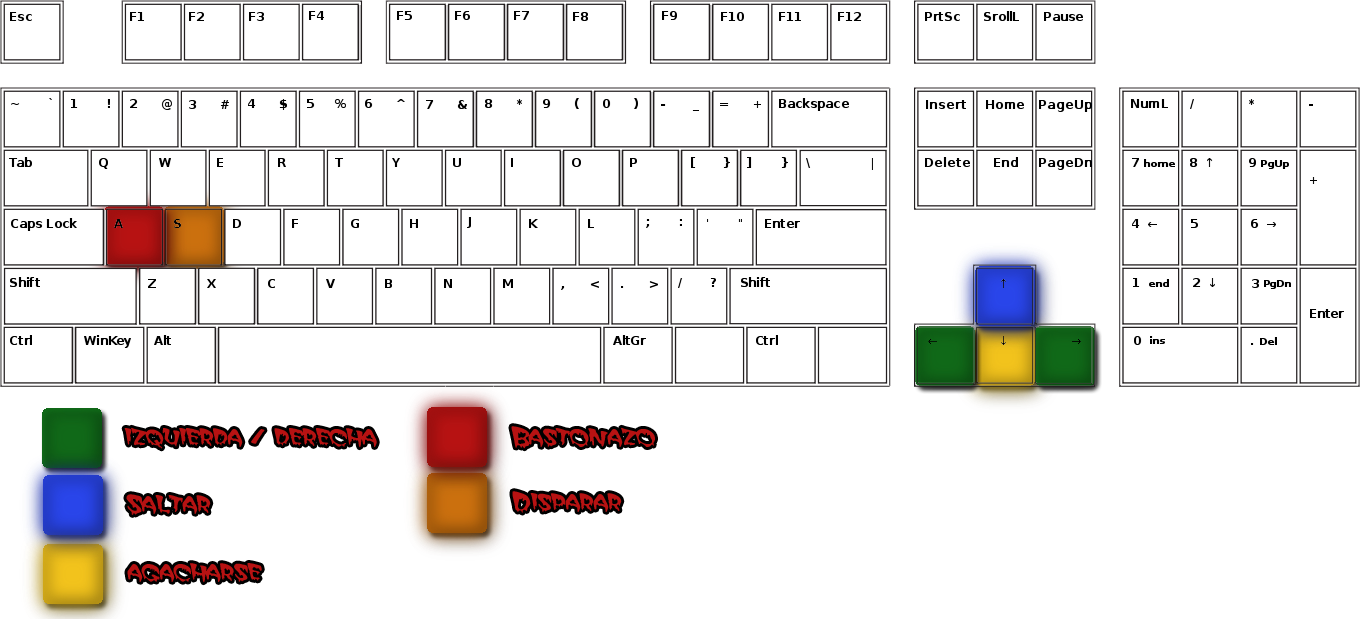
\includegraphics[scale=0.35]{controles.png}
\end{center}
